\documentclass{article}
\usepackage{geometry}
\geometry{left=2cm,right=2cm,top=2cm,bottom=2cm}

\usepackage{graphicx}
\graphicspath{{pics/}}

\setlength{\arrayrulewidth}{0.3mm}
\setlength{\tabcolsep}{18pt}
\renewcommand{\arraystretch}{1.3}

\usepackage{caption}
\usepackage{subcaption}
\usepackage{amsmath}
\begin{document}

\title{MACHINE LEARNING IN ROBOTICS \\ Assignment 2}
\author{Weiqi Luo \ 03697059}

\maketitle
\newpage

\section{Exercise 1}
\subsection{Learned GMM Parameters}
\begin{center}

\textbf{Component 1}
$$
\pi_1 = 0.2617 \quad
\mu_1=
\begin{bmatrix}
0.0262  \\  0.0617
\end{bmatrix}
\quad
\Sigma_1=
\begin{bmatrix}
0.0011 & -4.2436e-04 \\
-4.2436e-04  & 2.4312e-04
\end{bmatrix}
$$

\textbf{Component 2}
$$
\pi_2 = 0.2011 \quad
\mu_2=
\begin{bmatrix}
-0.0147 \\  -0.0796
\end{bmatrix}
\quad
\Sigma_2=
\begin{bmatrix}
3.9439e-04  & 2.1664e-04 \\
2.1664e-04  & 1.2757e-04
\end{bmatrix}
$$
	
\textbf{Component 3}
$$
\pi_3 = 0.2972 \quad
\mu_3=
\begin{bmatrix}
-0.0194 \\  -0.0166
\end{bmatrix}
\quad
\Sigma_3=
\begin{bmatrix}
   7.4372e-04 & -5.9168e-04 \\
   -5.9168e-04 &  6.1027e-04
\end{bmatrix}
$$

\textbf{Component 4}
$$
\pi_4 = 0.2400 \quad
\mu_4=
\begin{bmatrix}
-0.0432  \\  0.0446
\end{bmatrix}
\quad
\Sigma_4=
\begin{bmatrix}
1.7479e-04  & 2.6154e-04 \\
2.6154e-04  & 3.9754e-04
\end{bmatrix}
$$


\end{center}

\subsection{Visualization}
\begin{figure}[!ht]
	\centering
	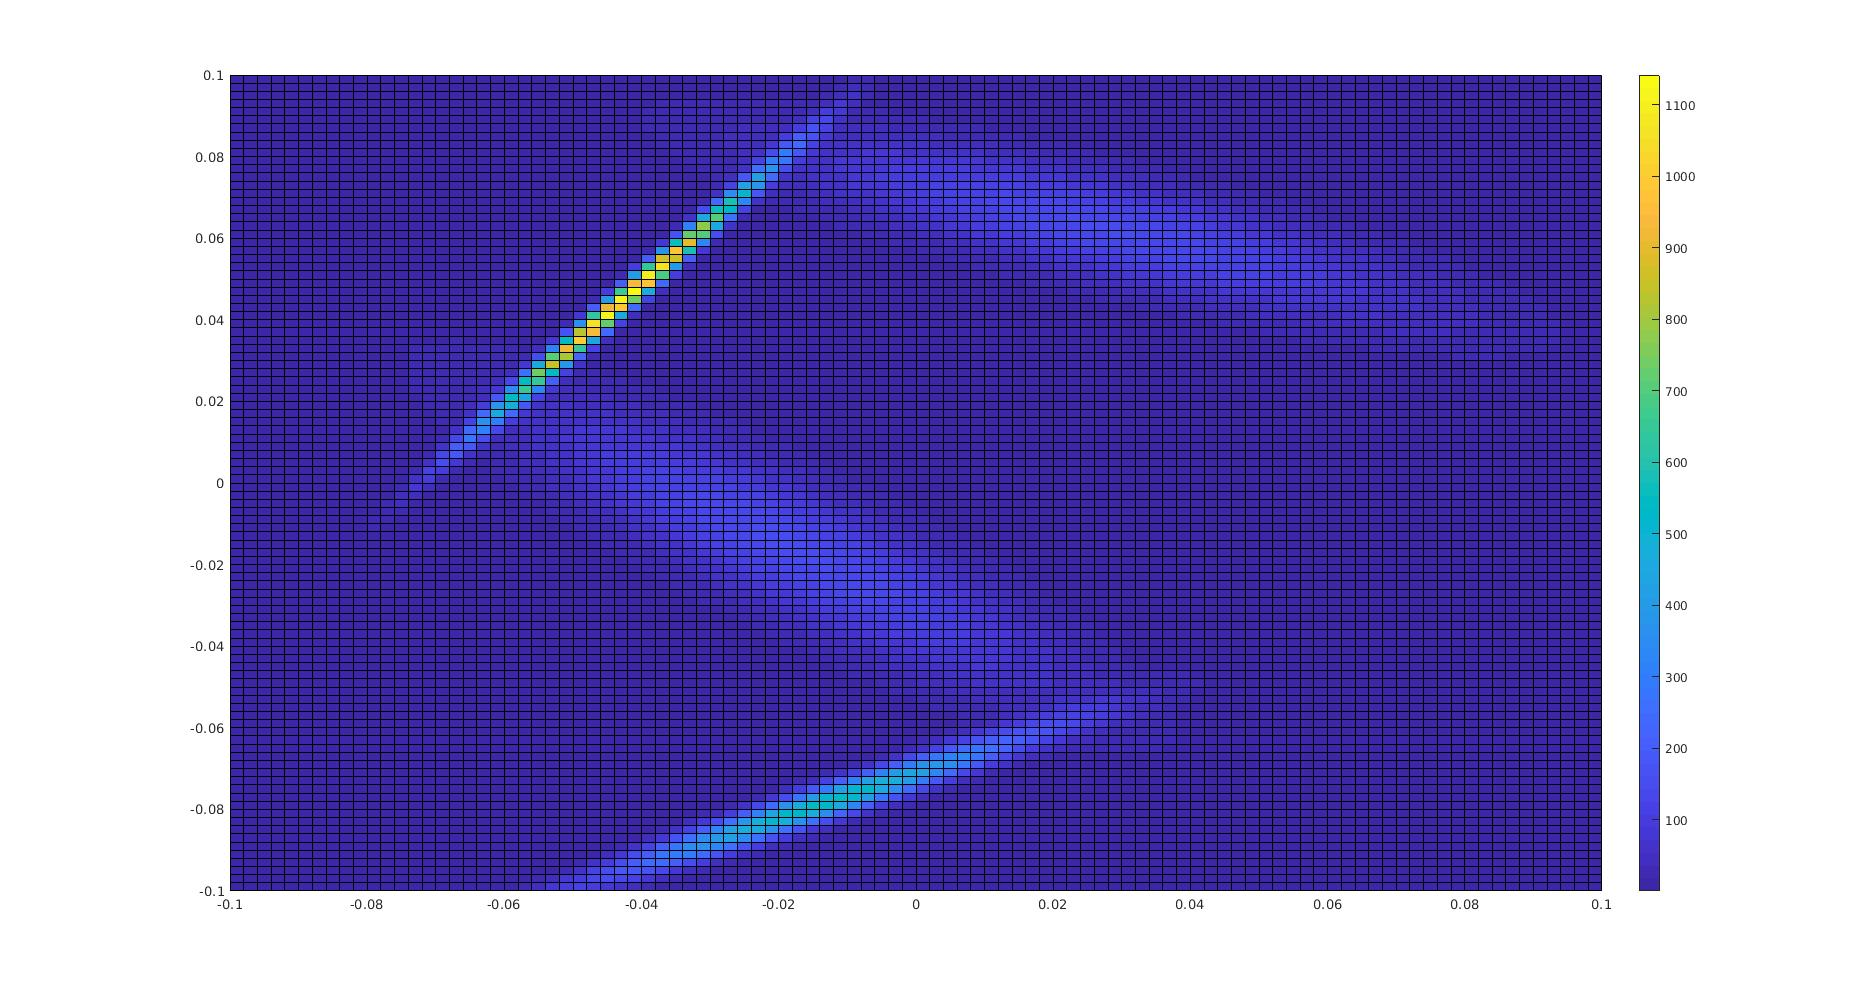
\includegraphics[width=1\linewidth]{1_3D.jpg} 
	\caption{GMM Density Function Visualization} 
\end{figure}
\newpage
\begin{figure}[ht]
	\centering
	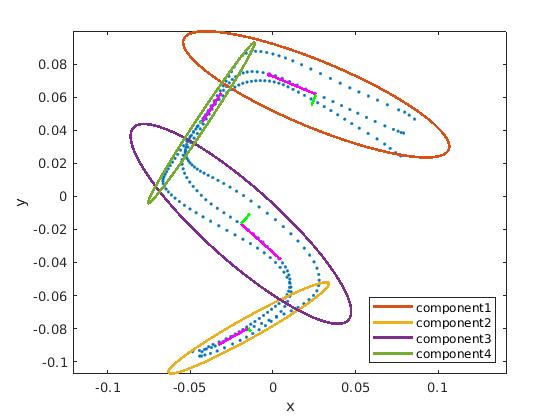
\includegraphics[width=0.8\linewidth]{1_2D.jpg} 
	\caption{GMM Components Visualization}  
\end{figure}


\newpage

\section{Exercise 2}
\subsection{Classification Result}
All sequences in Test.txt belong to gesture2.
\begin{center}
	\begin{tabular}{ c | c | c | c | c | c | c | c | c |c |c }
		\hline
		\textbf{Sequence} &1 & 2 &3 & 4&5 & 6&7 & 8&9 & 10\\
		\hline		
		\textbf{Label}  &2 & 2 &2 & 2&2 & 2&2 & 2&2 & 2 \\ \hline
	\end{tabular}
\end{center}

\subsection{Visualization}
\begin{figure}[ht]
	\centering
	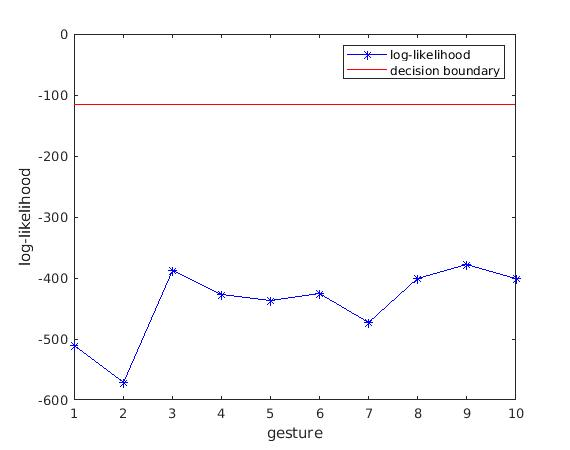
\includegraphics[width=1\linewidth]{EX2.jpg} 
	\caption{Log-likelihood visualization}  
\end{figure}

\newpage
\section{Exercise 3}
\subsection{Applying Policy Iteration}
\subsubsection{Report reward matrix}
\textbf{Positive Rewards:}
\\
- Moving the Robot forward
\\
\textbf{Negative Rewards:}
\\
- Moving a leg forward or backward while it is still on the ground
\\
- Raising one leg while the other is already in the air
\\
- Moving the Robot backward
\begin{center}
$$
Reward \ Matrix \ = \
\begin{bmatrix}		
0 & -1 & 0 & -1 \\
0 & 0 & -1 & -1 \\ 
0 & 0 & -1 & -1 \\ 
0 & -1 & 0 & -1 \\ 
-1 & -1 & 0 & 0 \\ 
0 & 0 & 0 & 0 \\ 
0 & 0 & 0 & 0 \\ 
-1 & 1 & 0 & 0 \\ 
-1 & -1 & 0 & 0 \\ 
0 & 0 & 0 & 0 \\ 
0 & 0 & 0 & 0 \\ 
-1 & 1 & 0 & 0 \\ 
0 & -1 & 0 & -1 \\ 
0 & 0 & -1 & 1 \\ 
0 & 0 & -1 & 1 \\ 
0 & -1 & 0 & -1 \\ 
\end{bmatrix}
$$	
\end{center}
\subsubsection{The choose of $\gamma$}
The discount factor $\gamma$ determines the importance of future rewards. A factor approaching 0 will make the agent short-sighted, while a factor of 0 will make it only considering current rewards, and the agent will fail to learn the optimal behavior. A factor approaching 1 will make it strive for a long-term high reward, however a large factor result in more iterations in oder to converge (see Fig.6). If the factor reaches 1 the resulting system of linear equations can not be solved because the matrix becomes singular.
\\ \\
I choose the value of $\gamma = 0.5$ according to Fig.6. 

\subsubsection{Iteration number}
The iteration number required for the policy iteration to converge is approximately between 2 and 7 according to Fig.6.

\newpage

\subsubsection{Experiments Result}
\paragraph{Initial State 10}
State sequence:	
10 ,    14 ,     2 ,     3 ,     4 ,     8 ,     5 ,     9 ,    13 ,    14 ,     2 ,     3 ,     4 ,     8 ,     5 ,     9.
\begin{figure}[ht]
	\centering
	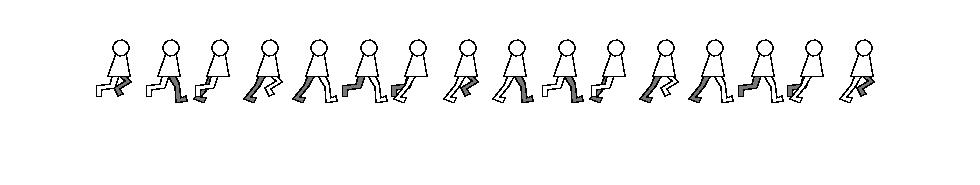
\includegraphics[width=1\linewidth]{policy_10.jpg} 
	\caption{Policy iteration with initial state 10}  	
\end{figure}
\paragraph{Initial State 3}
State sequence:	3  ,   4  ,   8  ,   5 ,    9 ,   13  ,  14 ,    2    , 3  ,   4  ,   8   ,  5   ,  9   , 13   , 14  ,   2.
\begin{figure}[ht]
	\centering
	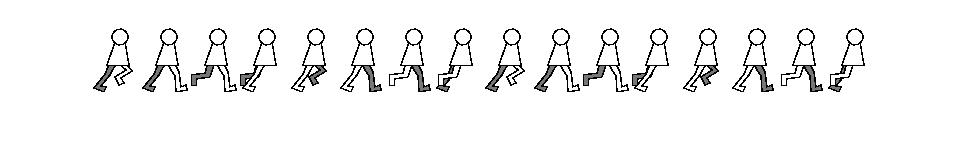
\includegraphics[width=1\linewidth]{policy_3.jpg} 
	\caption{Policy iteration with initial state 3}  	
\end{figure}

\begin{figure}[ht]
	\centering
	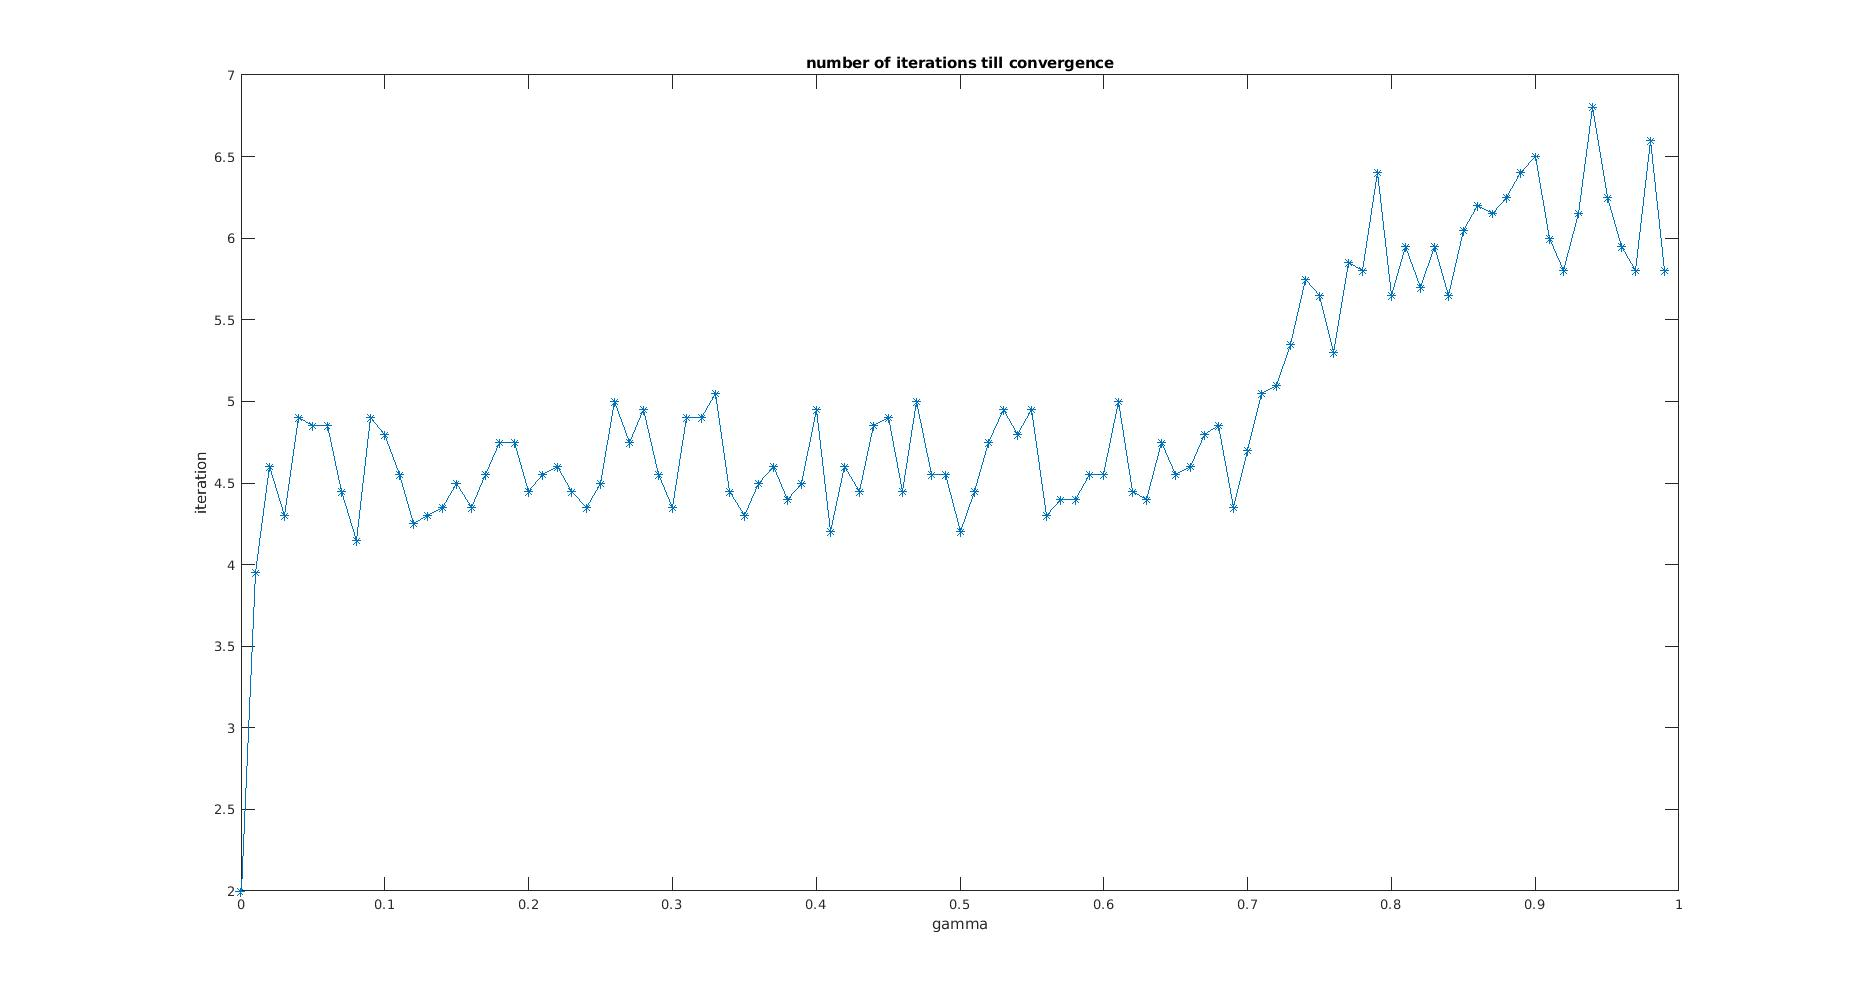
\includegraphics[width=0.8\linewidth]{iteration.jpg} 
	\caption{Average number of iterations for different discount factor $\gamma$}  	
\end{figure}

\newpage

\subsection{Applying Q-learning}
\subsubsection{The choose of $\epsilon$ and $\alpha$}
A learning rate $\alpha$ of 1 is selected. Since the reward and state transition matrix are deterministic, there is no need to consider several observations to incrementally approximate the average over all possible state. 
\\ \\
A linearly decreasing $\epsilon$ is chosen to speed up the convergence. At beginning $\epsilon=1$, which corresponds to a pure random policy, since the agent has no idea about the environment. As the agent collects more and more evidence, the policy shift towards a pure greedy policy.
\begin{figure}[ht]
	\centering
	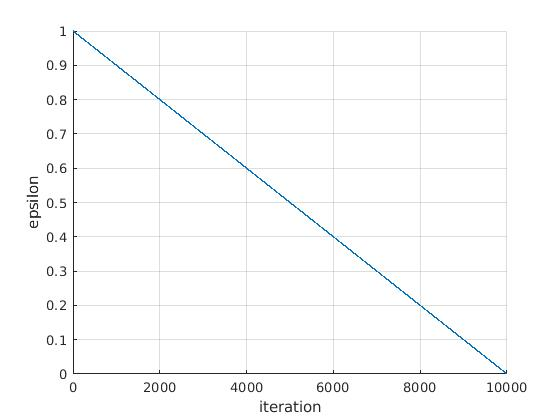
\includegraphics[width=0.7\linewidth]{line.jpg} 
	\caption{linearly decreasing $\epsilon$ with iteration}  	
\end{figure}  

\subsubsection{Compare of pure greedy policy and $\epsilon$-greedy}
In the case of pure greedy policy, the agent always performs the action witch correspond to the largest action-value function, no exploration is made by the algorithm. The learned policy will fail to converge at at the optimal policy.
\\ \\
If $\epsilon$ is too small, the system will fail to converge at at the optimal policy. If it is too large, it will take too many iterations to converge. A reasonable choise is to set $\epsilon$ decreasing with the number of iterations.

\subsubsection{Iteration numbers}
Approximately 1000
\newpage
\subsubsection{Experiments Result}
\paragraph{Initial State 5}
State sequence:	
 5   ,  9  ,  13   , 14   ,  2 ,    3  ,   4   ,  8  ,   5  ,   9  ,  13  ,  14  ,   2  ,   3   ,  4 ,    8.
\begin{figure}[ht]
	\centering
	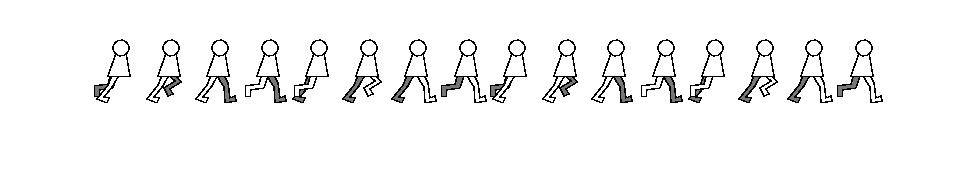
\includegraphics[width=1\linewidth]{Q_5.jpg} 
	\caption{Q learning with initial state 5}  	
\end{figure}
\paragraph{Initial State 12}
State sequence:	12   ,  9  ,  13 ,   14   ,  2   ,  3   ,  4  ,   8  ,   5  ,   9  ,  13 ,   14,     2  ,   3   ,  4   ,  8.
\begin{figure}[ht]
	\centering
	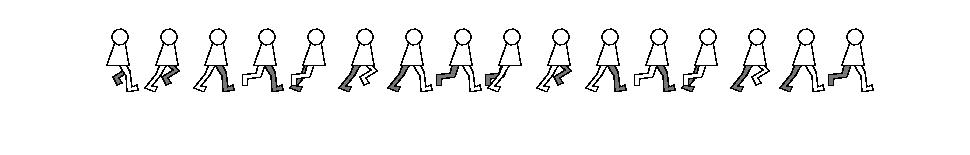
\includegraphics[width=1\linewidth]{Q_12.jpg} 
	\caption{Q learning with initial state 12}  	
\end{figure}

\end{document}